\documentclass{controle}
\usepackage{main}

\title{Automatismes n°2}
\date{}
\author{Première Spécialité Mathématiques}

\begin{document}
\titleonly{}
\begin{tcolorbox}
Répondre aux questions à choix multiples suivantes. Plusieurs réponses sont possibles par question.
\end{tcolorbox}
\begin{questions}
\question Laquelle de ces fractions est égale à $\dfrac{15}{16}$ :

\begin{oneparchoices}
\choice $\dfrac{7}{8} \times \dfrac{1}{2}$
\choice $\dfrac{7}{8} + \dfrac{1}{2}$
\choice $\dfrac{7}{8} \div \dfrac{1}{2}$
\choice $\dfrac{7}{8} - \dfrac{1}{2}$
\end{oneparchoices}

\question Lequel de ces nombres est égal à $35^3$ ?

\begin{oneparchoices}
\choice $3^3 \div 7^{-3}$
\choice $3^3 \times 7^3$
\choice $3^{-3} \div 7^3$
\choice $(-3)^3 \times (-7)^3$
\end{oneparchoices}

\question Lequel de ces nombre vaut $0,33$ ?

\begin{oneparchoices}
\choice $\dfrac{78}{254}$
\choice $3300000 \times 10^{-6}$
\choice $33\%$
\choice $\dfrac{3300}{10000}$
\end{oneparchoices}

\question Laquelle de ces distance correspond à \qty{4,7e3}{\meter} ?

\begin{oneparchoices}
\choice \qty{4,7e1}{\centi\meter}
\choice \qty{4,7e6}{\milli\meter}
\choice \qty{4,7e3}{\milli\meter}
\choice \qty{4,7e5}{\centi\meter}
\end{oneparchoices}

\question Soit $c$ un entier naturel. Quelle expression est égale à l'inverse du triple de l'entier naturel suivant $c$ ?

\begin{oneparchoices}
\choice $\dfrac{3}{(c+1)}$  
\choice $\dfrac{1}{3(c+1)}$
\choice $\dfrac{1}{3c}+1$
\choice $\dfrac{1}{3c}+\dfrac{1}{3}$
\end{oneparchoices}

\question Quelle expression est la forme développée réduite de $(6x + 3)^2$ ?

\begin{oneparchoices}
\choice $36x^2 + 18x + 9$
\choice $18x^2 + 36x + 9$
\choice $18x + 36x^2 + 9$
\choice $36x + 18x + 9$
\end{oneparchoices}

\question Quelle expression est une forme factorisée de $28x^2 + 56x$ ?

\begin{oneparchoices}
\choice $2x(14x + 28x)$
\choice $7(4x^2 + 8x)$
\choice $4x(7x + 14)$
\choice $x(28x^2 + 56)$
\end{oneparchoices}

\question Soient $a; b; c; d; f$ des nombres réels tels que $f = \dfrac{a - b}{c + d}$ et $c + d \neq 0$. Quelle expression est égale à $d$ ?

\begin{oneparchoices}
\choice $\dfrac{a - b}{f} - c$
\choice $\dfrac{a + b}{f} - c$  
\choice $\dfrac{a - b}{f} + c$  
\choice $\dfrac{a + b}{f} + c$  
\end{oneparchoices}

\question Quel est l'ensemble des solutions de $(4x + 8)(-x + 12) ?$

\begin{oneparchoices}
\choice $\varnothing$
\choice $\set{12;-2}$
\choice L'ensemble des solutions de $(4x + 8)(3x - 36)$
\choice $\set{-2;12}$
\end{oneparchoices}

\question $20\%$ du public d'un concert représente \num{1206} personnes. Combien y a-t-il de personnes à ce concert ?

\begin{oneparchoices}
\choice \num{6003}
\choice \num{6300}
\choice \num{6000,3}
\choice \num{6030}
\end{oneparchoices}

\question Augmenter de $12\%$ revient à multiplier par \dots

\begin{oneparchoices}
\choice $1,12$
\choice $0,12$
\choice $0,88$
\choice $1 + \dfrac{1}{12}$
\end{oneparchoices}

\question Après augmentation de $40\%$, le prix de mon pull est \num{120}€. Quel calcul faire pour retrouver le prix initial ?

\begin{oneparchoices}
\choice $\dfrac{120 \times 6}{5}$
\choice $\dfrac{120}{1,40}$
\choice $\dfrac{120 \times 5}{6}$
\choice $\dfrac{1,40}{120}$
\end{oneparchoices}

\question Quelle formule correspond au taux d'évolution en pourcentages la valeur $V_d$ à $V_f$ ?

\begin{oneparchoices}
\choice $\dfrac{V_d - V_f}{V_d} \times 100$
\choice $\dfrac{V_f - V_d}{V_d} \div 100$
\choice $\dfrac{V_f - V_d}{V_d} \times 100$
\choice $\dfrac{V_f - V_d}{V_f} \times 100$
\end{oneparchoices}

\question On augmente un prix de $10\%$, puis on diminue ce nouveau prix de $10\%$. Quel est le taux d'évolution global en pourcentages du prix ?

\begin{oneparchoices}
\choice $0\%$
\choice $-1\%$
\choice $+1\%$
\choice $+99\%$
\end{oneparchoices}

\question On augmente un prix de $25\%$. Comment calculer le taux d'évolution réciproque, qui correspond au taux d'évolution du nouveau prix vers le prix initial ?

\begin{oneparchoices}
\choice $\dfrac{1}{0,25} + 1$
\choice $\dfrac{1}{1,25} - 1$
\choice $\dfrac{1}{0,25} - 1$
\choice $\dfrac{1}{0,75} - 1$
\end{oneparchoices}

\question La courbe représentative d'une fonction $f$ est représentée ci-après. Lequel des nombres suivant est un antécédant de $2$ ?

\begin{center}
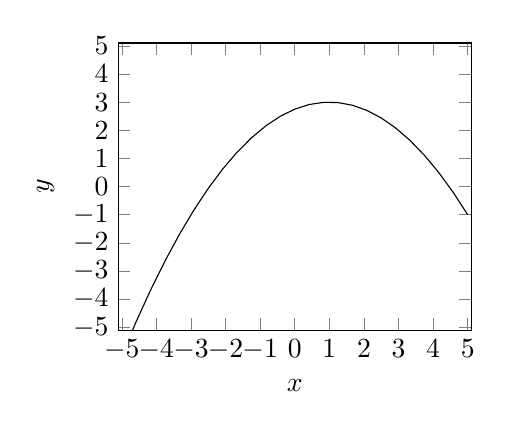
\begin{tikzpicture}
\begin{axis}
  [width = 0.5\textwidth,
  xlabel = $x$,
  ylabel = $y$,
  xmin = -5.1, xmax=5.1,
  ymin = -5.1, ymax=5.1,
  xtick distance=1,
  ytick distance=1]
\addplot [domain=-5:5] {-0.25*(x-1)^2 + 3};
\end{axis}
\end{tikzpicture}
\end{center}

\begin{oneparchoices}
\choice $3$
\choice $-1$
\choice $-3$
\choice $1$
\end{oneparchoices}

\question La courbe $\mathcal{C}$ est définie par l'équation $y = x^2 - 8x + 7$. Lequel de ces points est un point d'intersection entre $\mathcal{C}$ et l'axe des abscisses ?

\begin{oneparchoices}
\choice $A(7;0)$
\choice $B(0;7)$
\choice $C(1;0)$
\choice $D(-8;0)$
\end{oneparchoices}

\question Soit $f \colon x \mapsto -6x - 1$ définie sur $\R$. Laquelle de ces courbes représentées ci-après est la courbe représentative de $f$ ?

\begin{center}
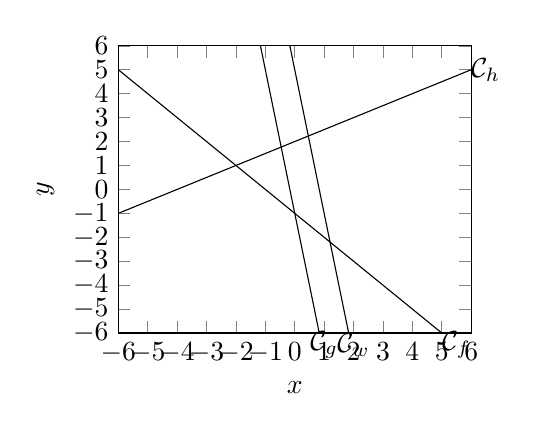
\begin{tikzpicture}
\begin{axis}
  [width = 0.5\textwidth,
  xlabel = $x$,
  ylabel = $y$,
  xmin = -5, xmax=5,
  ymin = -5, ymax=5,
  xtick distance=1,
  ytick distance=1,
  enlargelimits=true,
  clip mode=individual
  ]
\addplot[domain=-6:5]{-x - 1};
\draw (5.5,-6.5) node {$\mathcal{C}_f$};
\addplot [domain=-6:5]{-6*x - 1};
\draw (1,-6.5) node {$\mathcal{C}_g$};
\addplot[domain=-6:6] {0.5*x+2};
\draw (6.5,5) node {$\mathcal{C}_h$};
\addplot[domain=-6:6] {-6*x+5};
\draw (2,-6.5) node {$\mathcal{C}_w$};
\end{axis}
\end{tikzpicture}  
\end{center}

\begin{oneparchoices}
\choice $\mathcal{C}_f$
\choice $\mathcal{C}_g$
\choice $\mathcal{C}_h$
\choice $\mathcal{C}_w$
\end{oneparchoices}

\question Une droite passe par les deux points $A(3,4)$ et $B(7,9)$. Quel est sont coefficient directeur ?

\begin{oneparchoices}
\choice $\dfrac{7 - 3}{9 - 4}$
\choice $\dfrac{9 - 7}{4 - 3}$
\choice $\dfrac{9 - 4}{7 - 3}$
\choice $\dfrac{4 - 9}{7 - 3}$
\end{oneparchoices}
\end{questions}
\end{document}